%
% chap002.tex
%

\chapter{Die Summe der ersten $n$ natürlichen Zahlen}

Das einfachste Muster ist, dass die Steine in einer
rechtwinkligen Dreiecksform angeordnet sind und die
Anzahl der Steine von oben nach unten jeweils um eins
zunimmt.

Es stellt sich hier die Frage, was die Summe
$1+2+3+\dots+10$ beträgt?

Zur Beantwortung dieser Frage betrachtet man die Figur
in folgender Abbildung~\ref{fig:muster_gauss_summe}.
Dabei legt man die blauen Steine in 
einer rechtwinkliger Dreicksform von oben nach unten
in aufsteigender Anzahl aus. Danach verdoppelt man
die Figur, indem man gleich viele rote Steine von
unten nach oben in absteigender Anzahl legt.
Dadurch bekommt man ein rechteckiges Muster mit
insgesamt $10 \cdot 11 = 110$ Steinen.
Das gesuchte Ergebnis ist:
$\frac{1}{2} \cdot 110 = 55$

\begin{figure}[H]
  \centering
  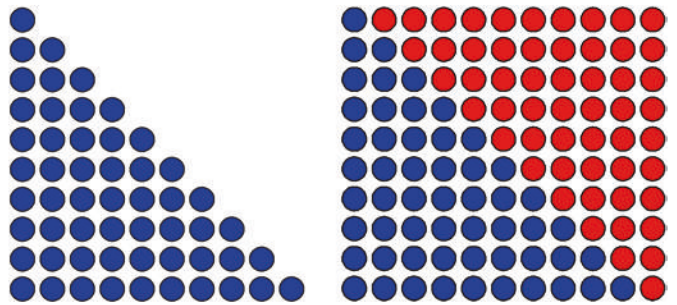
\includegraphics[width=.5\linewidth]{./images/muster02.png}
  \caption[Muster aus bunten Steinen in Dreicksform]{Muster aus bunten Steinen in Dreicksform}
  \label{fig:muster_gauss_summe}
\end{figure}

\textbf{Die Summenformel der ersten $n$ natürlichen Zahlen:}
\[
  1 + 2 + 3 + \dots + n = \frac{1}{2} \cdot n \cdot (n+1) 
\]

Mit der Gaußschen Summenformel lässt sich die Summe aller natürlichen Zahlen bis zu einer Obergrenze $n$ berechnen. Sie lautet:
\[
  \sum_{i=1}^{n} i = \frac{n\cdot(n+1)}{2}
\]

\begin{proof}[\textbf{Beweis durch vollständige Induktion}]
 $\text{}$
 
 \begin{itemize}
  \item Induktionsanfang: $n = 1$
        \[
         \sum_{i=1}^{1} 1 = \frac{1}{2} \cdot 1 \cdot (1+1)
        \]
  \item Induktionsvoraussetzung:\\  
        Es gelte
        \[
         \sum_{i=1}^{n} i = \frac{1}{2} \cdot n \cdot (n+1)
        \]
  \item Induktionsschritt: $n = n + 1$
        \[
         \begin{array}{rcl}
           \sum\limits_{i=1}^{n+1} i
           & = & \sum\limits_{i=1}^{n} i + (n+1) \\\\
           & = & \dfrac{1}{2} \cdot n \cdot (n+1) + (n+1) \\\\
           & = & \dfrac{1}{2} \cdot (n+1) \cdot (n+2)
         \end{array}
        \]
 \end{itemize}
\end{proof}

\textbf{\textit{Aufgabe 2.1}:}
Bestimmen Sie systematisch die Summe der ersten $n$ natürlichen
Zahlen mit größtem Summanden $n = 1, 2, 3, \dots, 20$.

\textbf{\textit{Lösung}:}
\[
  \sum_{i=1}^{20} i = \frac{1}{2} \cdot 20 \cdot (20+1) = 210
\]


\textbf{\textit{Aufgabe 2.2}:}
Bis zu welcher natürlichen Zahlen n muss man summieren,
bis die Summe $100$ [$1000$; $1.000.000$] überschritten wird?

\textbf{\textit{Lösung}:}
Man muss bis zu den natürlichen Zahlen $14$, $45$
und $1414$ jeweils summieren, bis die Summe $100$, $1000$
und $1.000.000$ überschritten wird.








